\chapter{Examples of use of the \glyph{equivalence operator}}
\label{ex_eq}

In the following, we give examples of use and misuse of the newly introduced \glyph{equivalence operator} (\sect{equivalence}).

Figures~\ref{fig:D1_2} and~\ref{fig:D1_3} introduce the use of the \glyph{equivalence operator} to form generic \glyph{EPNs}.
They show how the use of such an operator might allow reducing drastically the complexity of a map, without losing any information.

\begin{figure}
    \centering
    \begin{tabular}{lc}
        A & \raisebox{-\height}{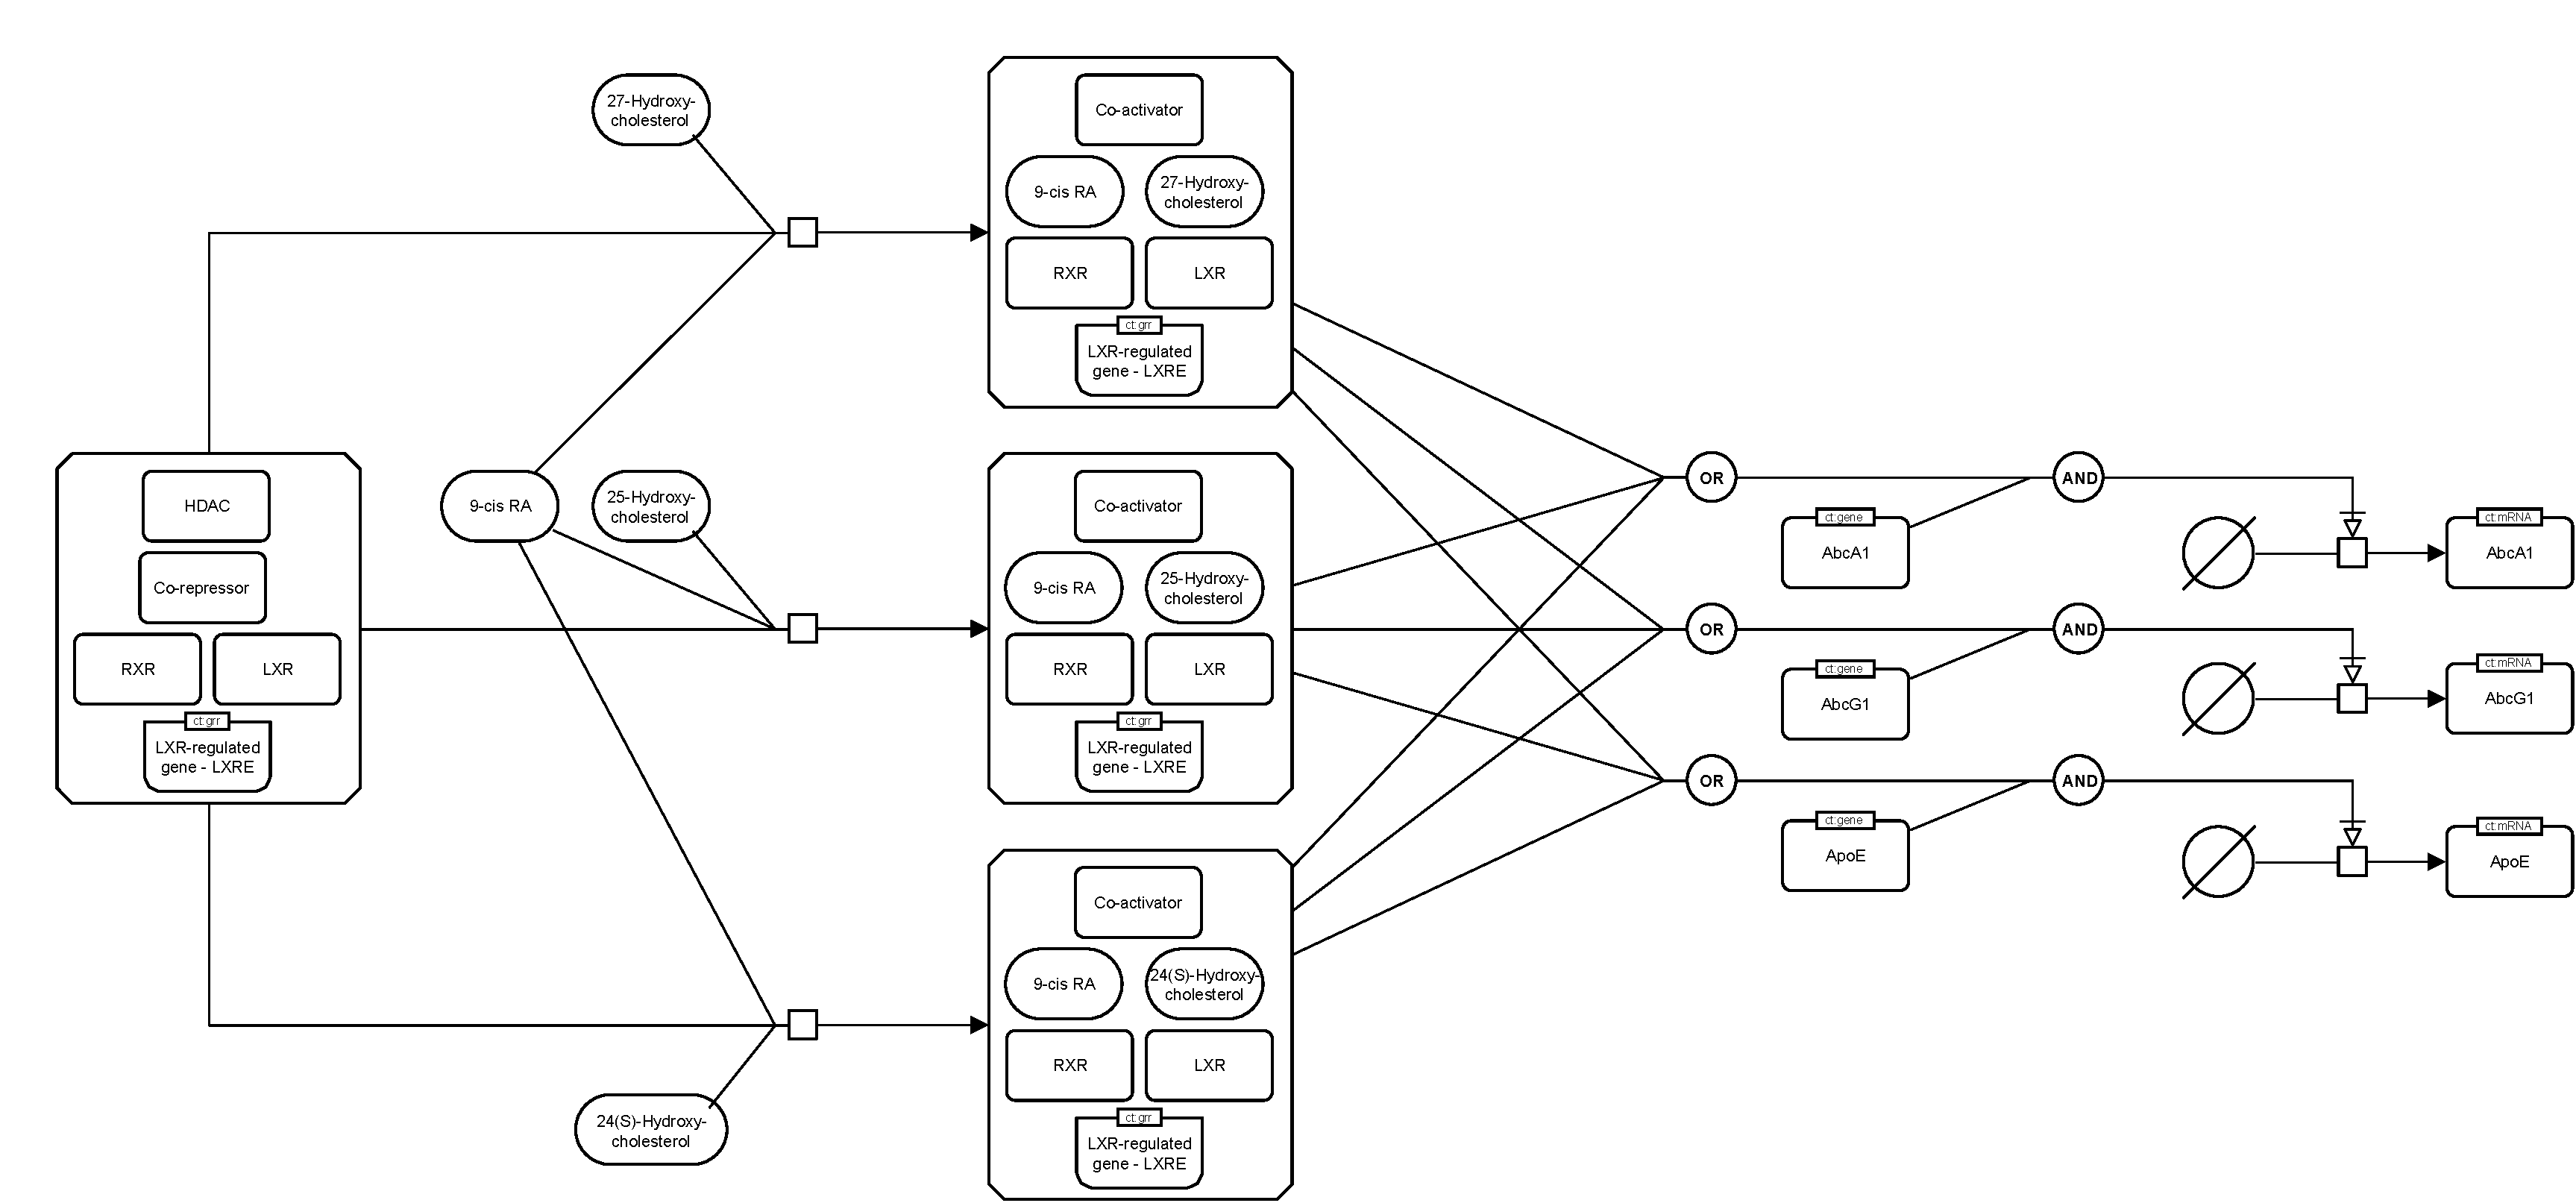
\includegraphics[scale=0.25]{examples/D1_2A}}\\
        B & \raisebox{-\height}{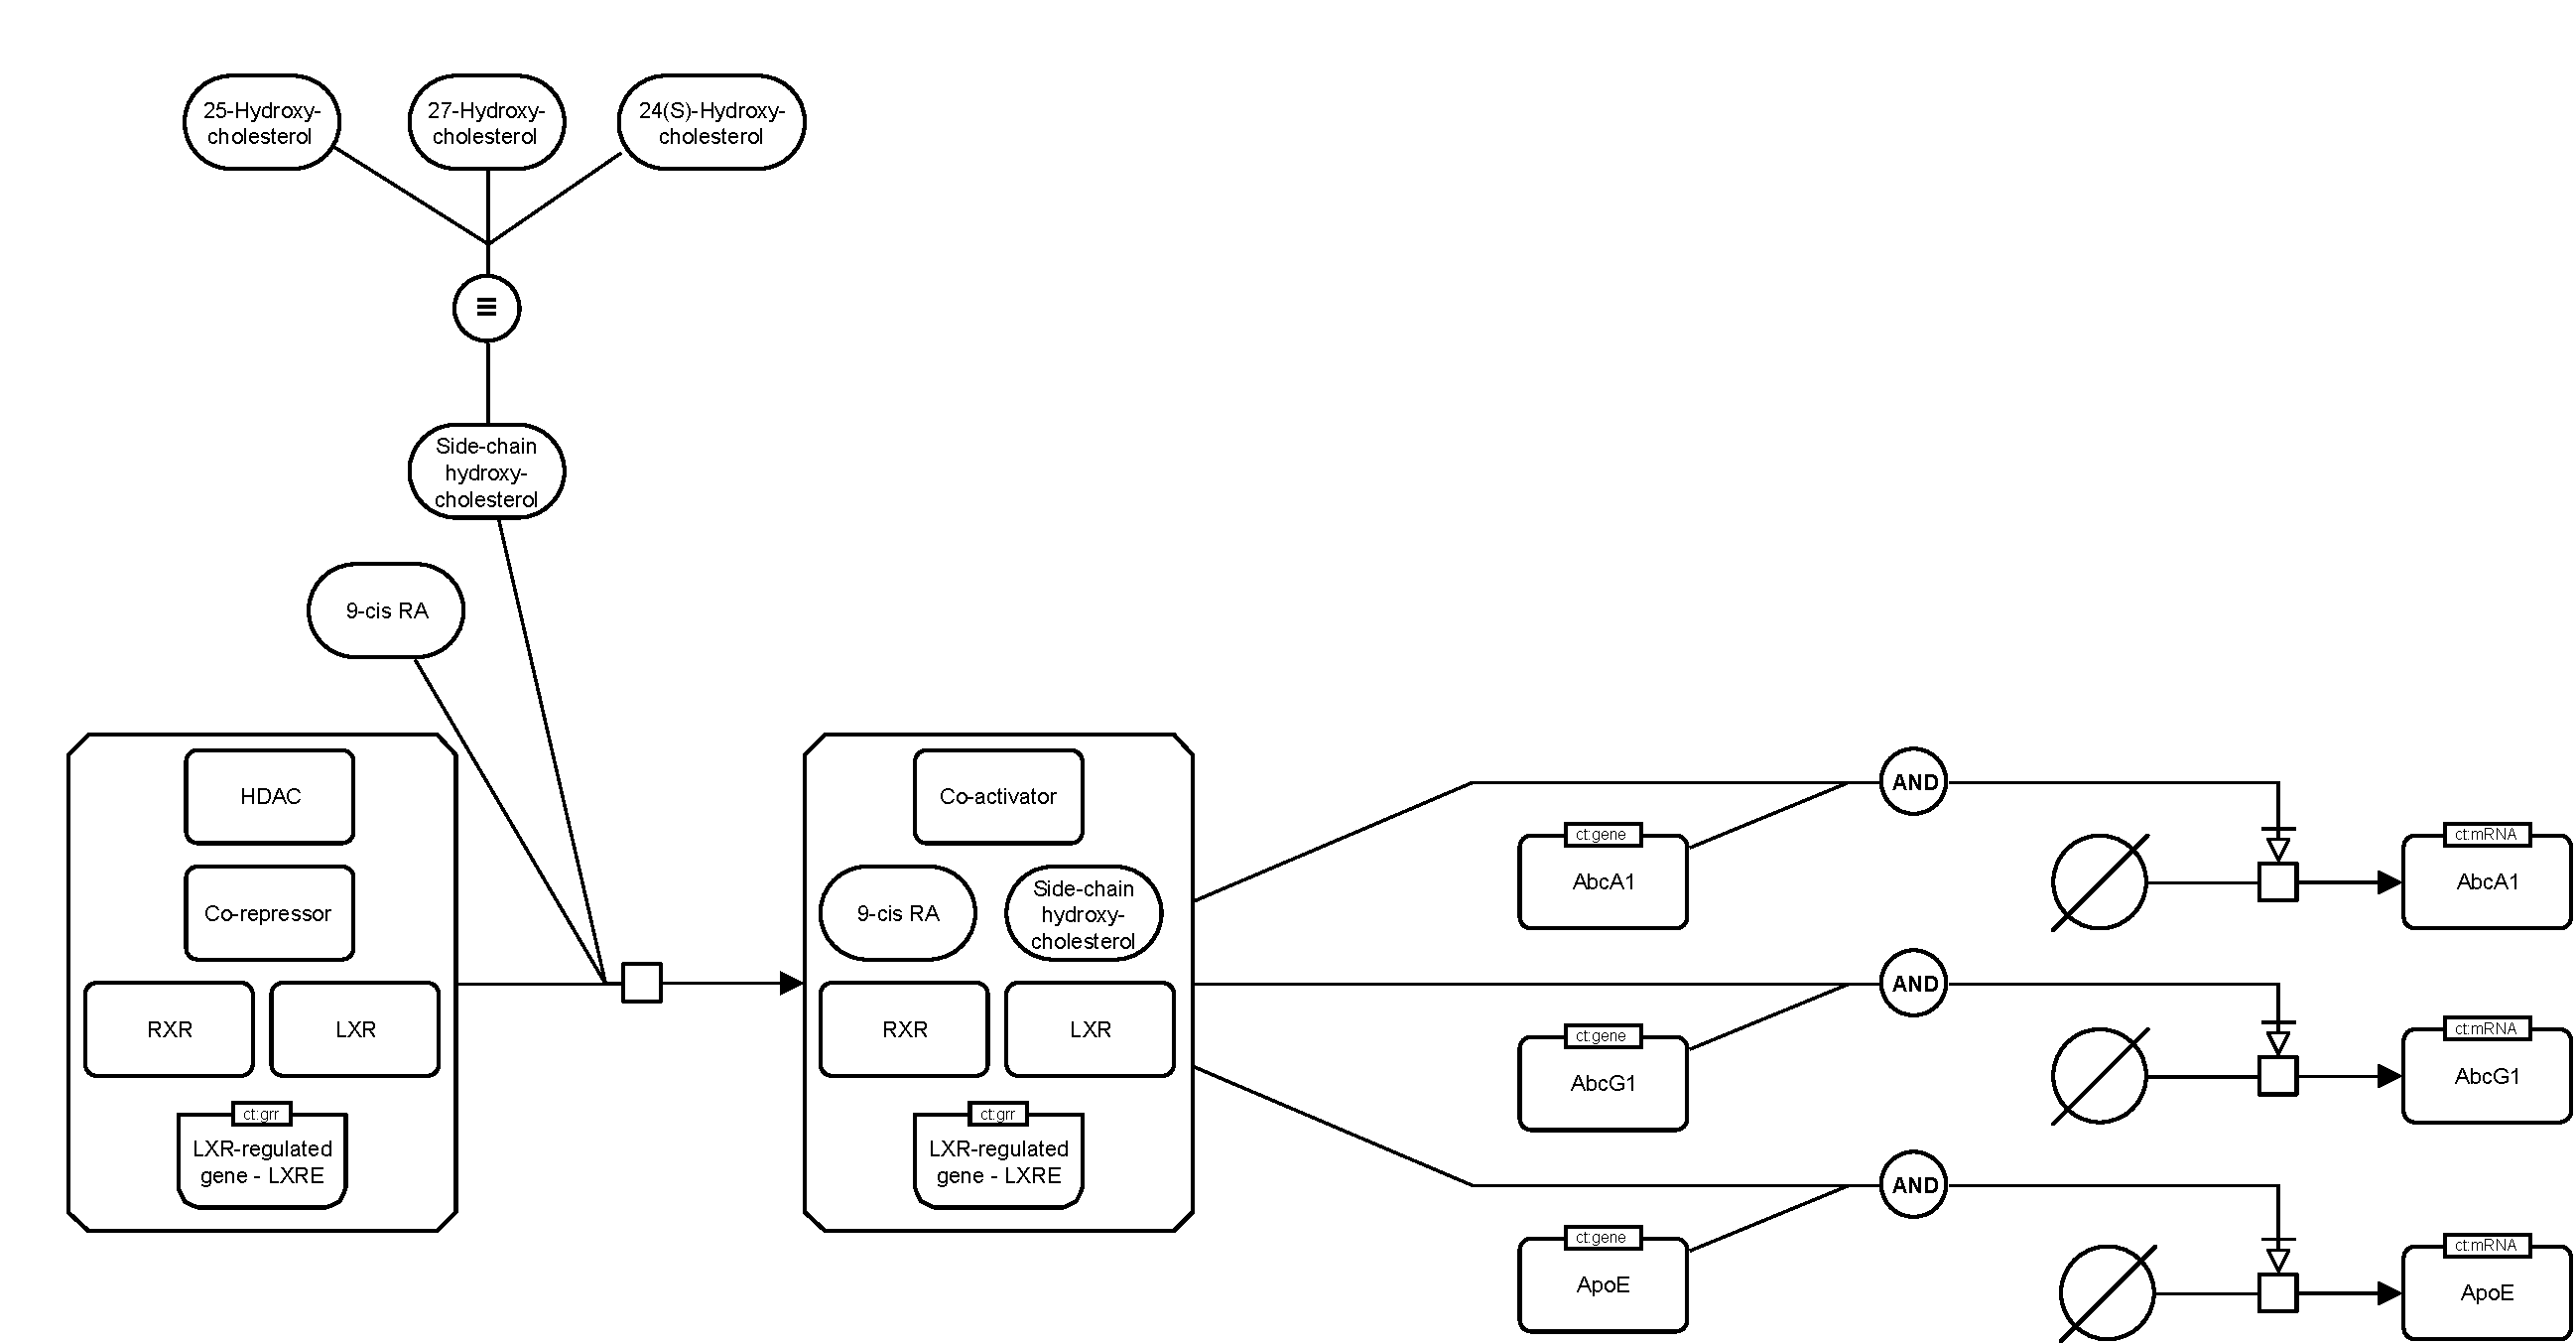
\includegraphics[scale=0.25]{examples/D1_2B}}
\end{tabular}
\caption{LXR signalling induced by 25-hydroxycholesterol, 27-hydroxycholesterol and 24(S)-hydroxycholesterol. A. Without an \glyph{equivalence operator}: events have to be multiplied for the three hydroxysterols. B. With an \glyph{equivalence operator}: a compact representation is possible allowing a better readability.}
\label{fig:D1_2}
\end{figure}

\begin{figure}
    \centering
    \begin{tabular}{lc}
        A & \raisebox{-\height}{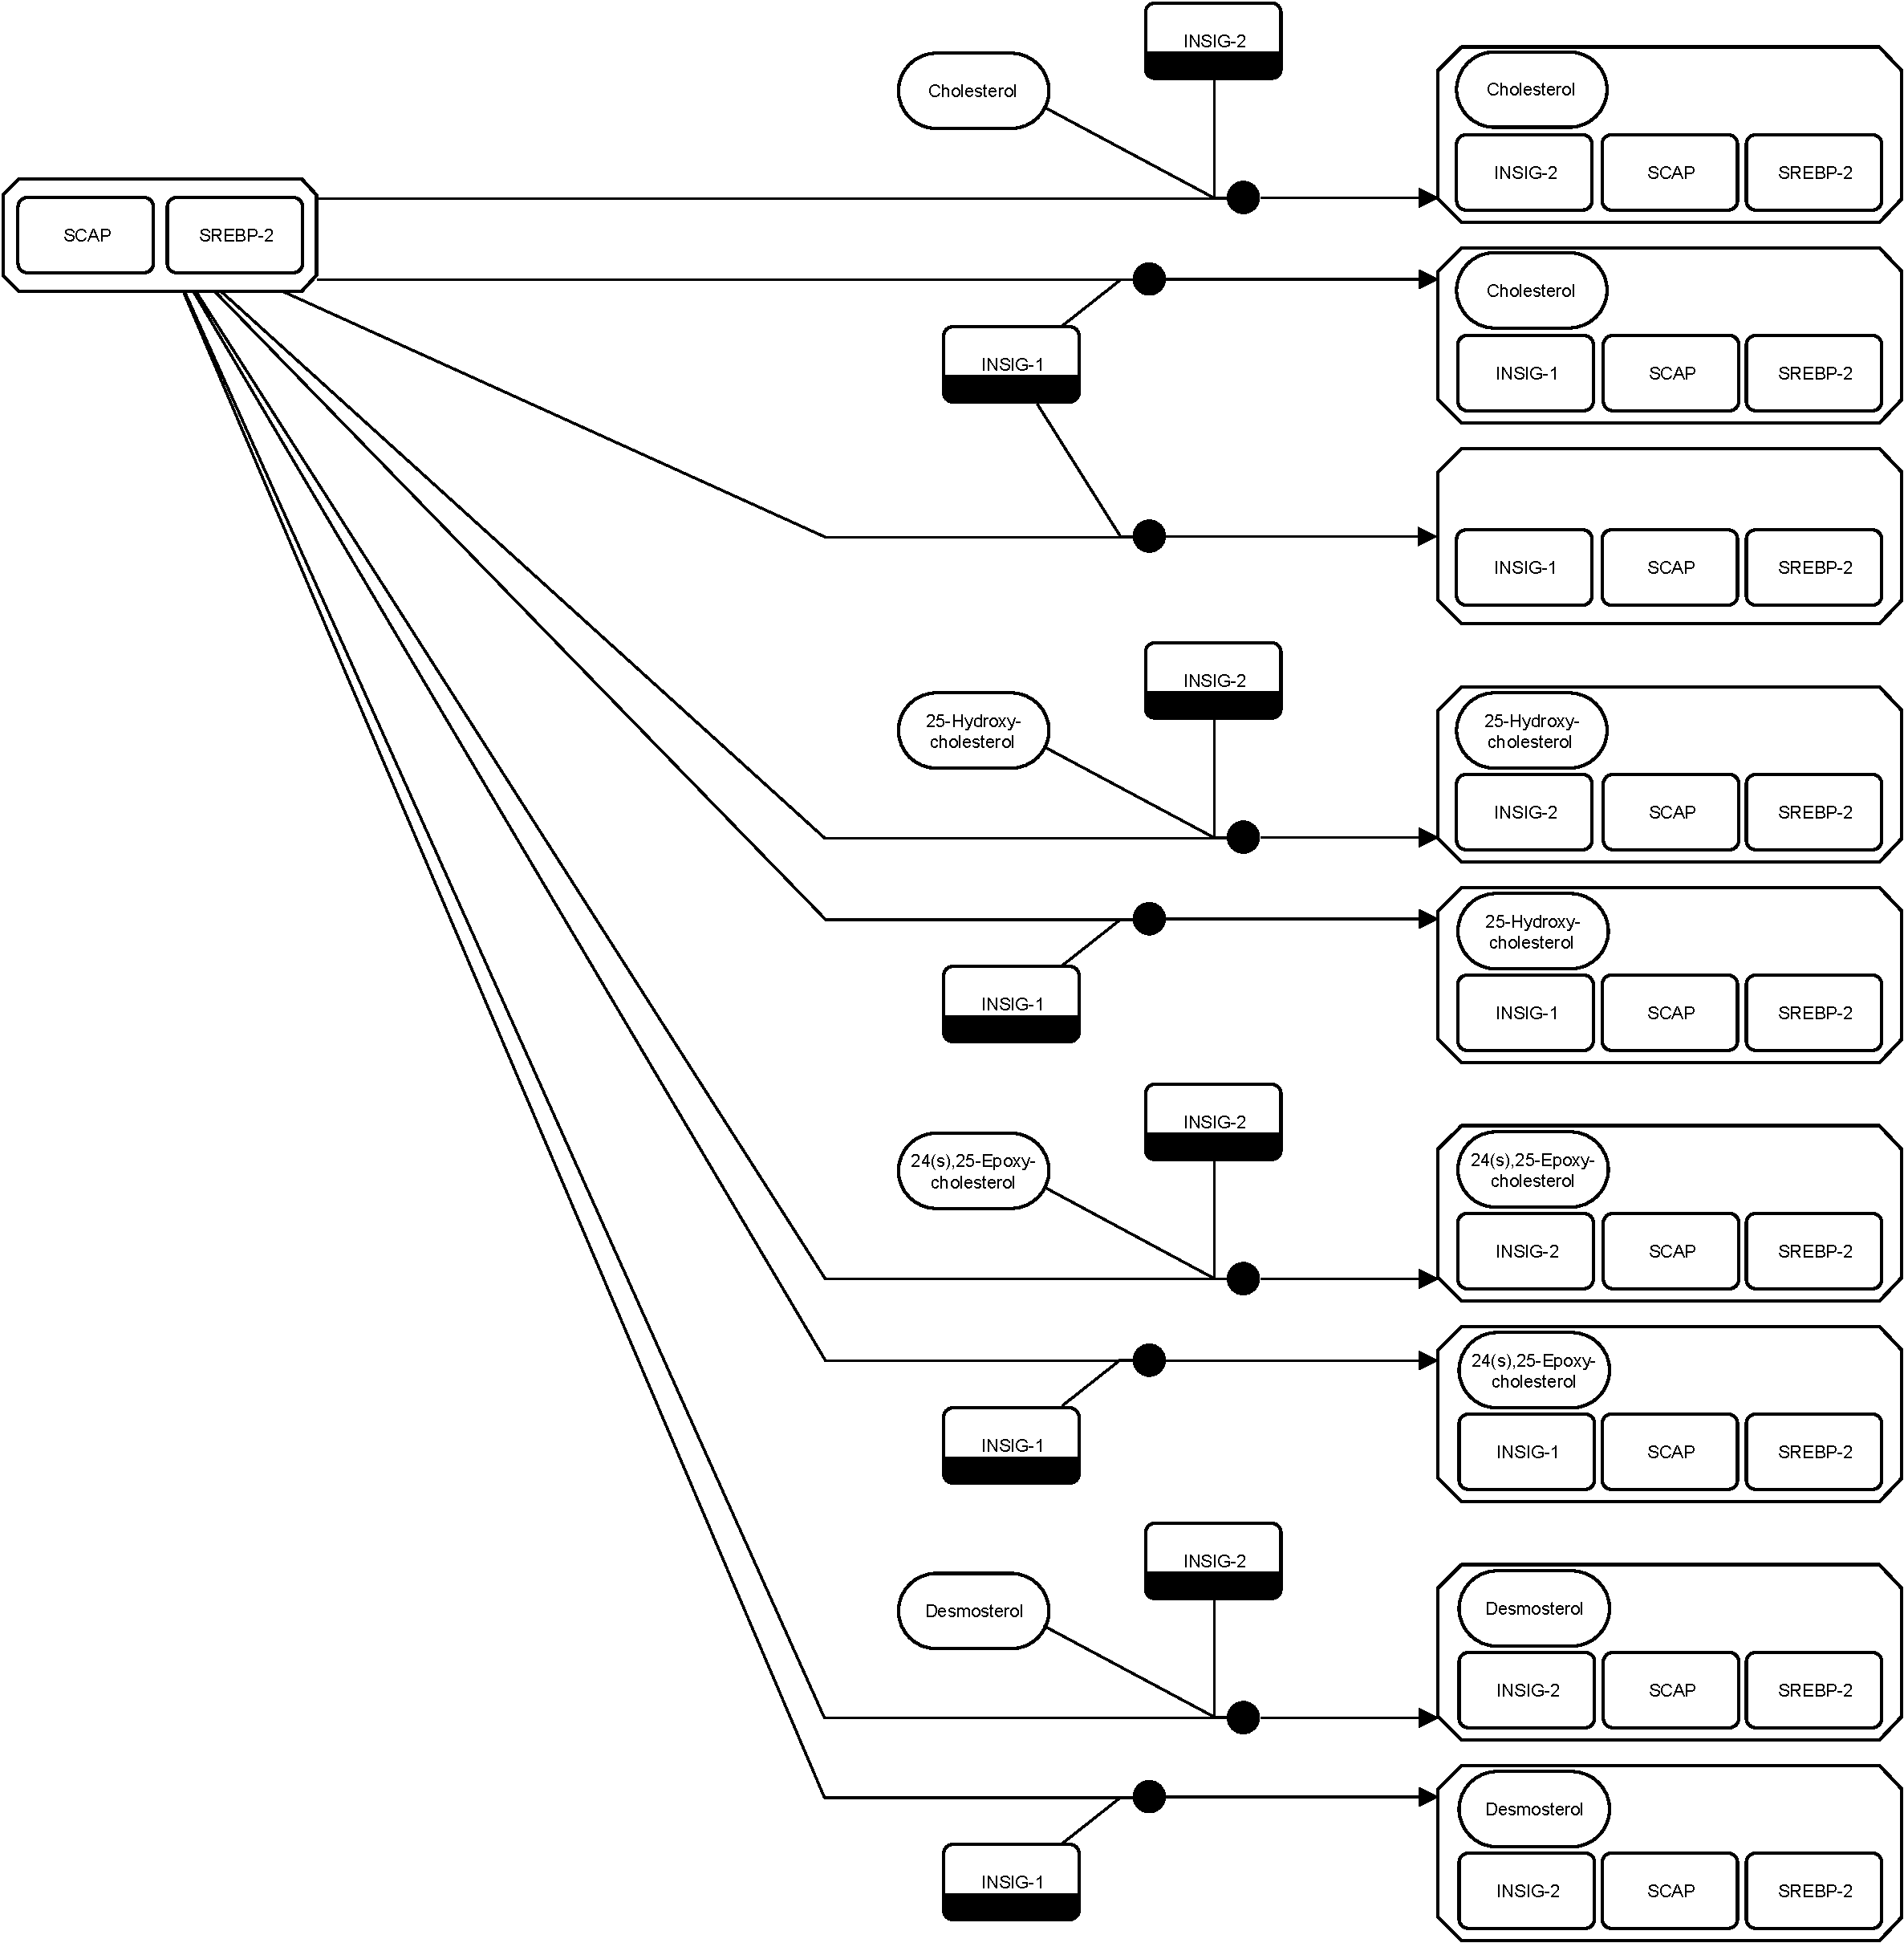
\includegraphics[scale=0.35]{examples/D1_3A}}\\
        B & \raisebox{-\height}{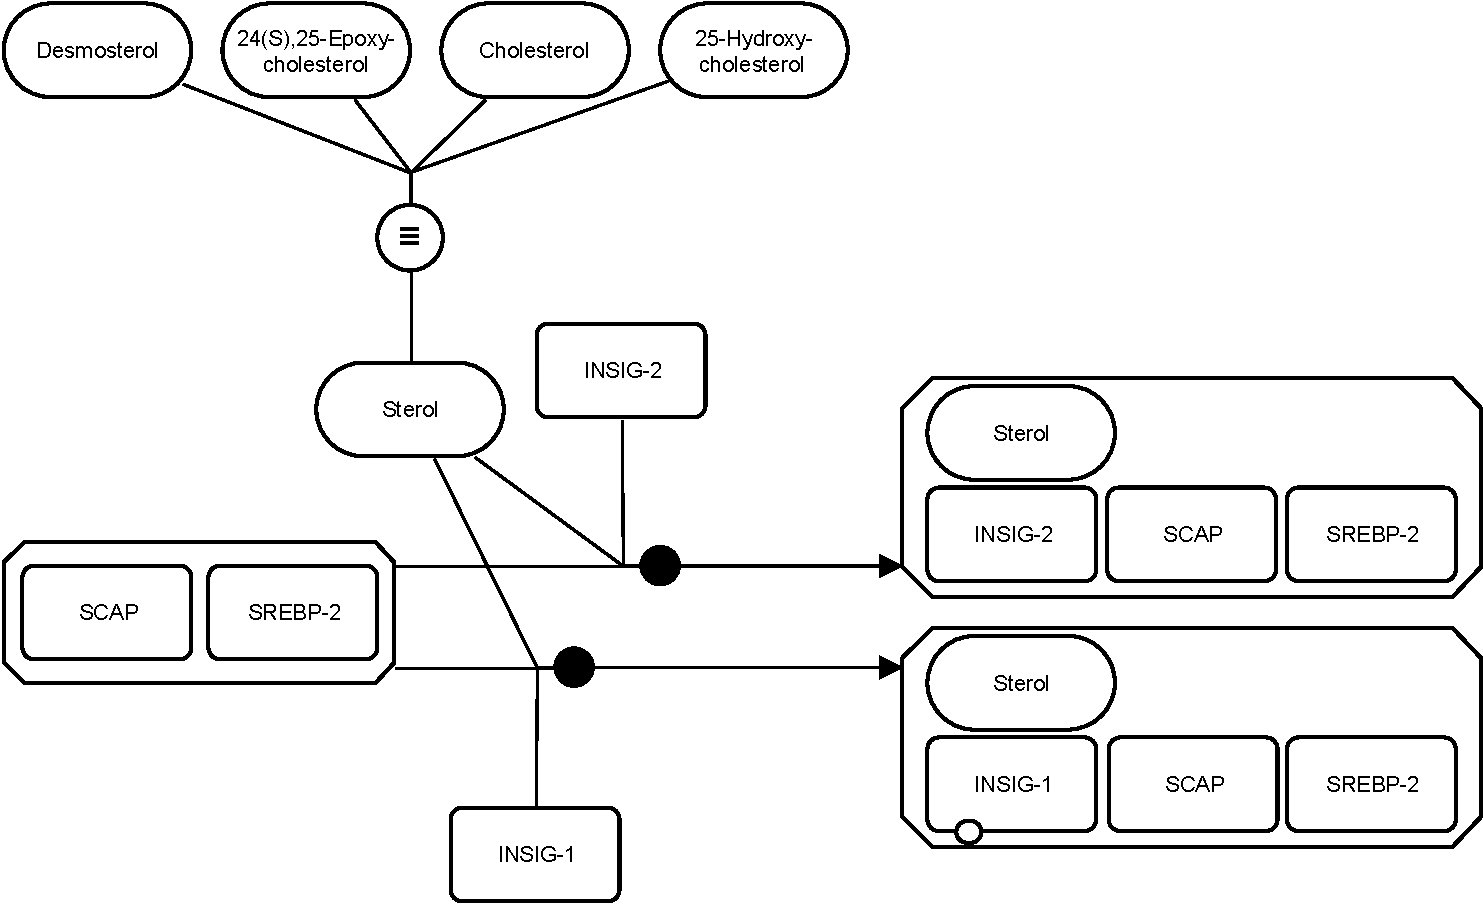
\includegraphics[scale=0.35]{examples/D1_3B}}
    \end{tabular}
\caption{First step of the inhibition of cholesterol synthesis in presence of sterols. A. Without an \glyph{equivalence operator}. B. With an \glyph{equivalence operator}.}
\label{fig:D1_3}
\end{figure}

Figures~\ref{fig:D3_3}, \ref{fig:D3_1}, and~\ref{fig:D3_2} show misuses of the \glyph{equivalence operator}.
The use of the \glyph{equivalence operator} requires respecting a number of rules (\sect{eq-semantics}), that we recall briefly here: 1. Pools should not overlap; 2. A \glyph{process} should not affect \glyph{EPNs} belonging or deriving from both sides of an \glyph{equivalence operator}; 3. For \glyph{simple chemicals} (stateless \glyph{EPNs}) it is not allowed to show specifics both as input and as output of a pathway.
The example of \fig{D3_3} does not respect the first rule, the example of \fig{D3_2} does not respect the first two rules, and the example of \fig{D3_2} does not respect the third rule.

\begin{figure}
\begin{center}
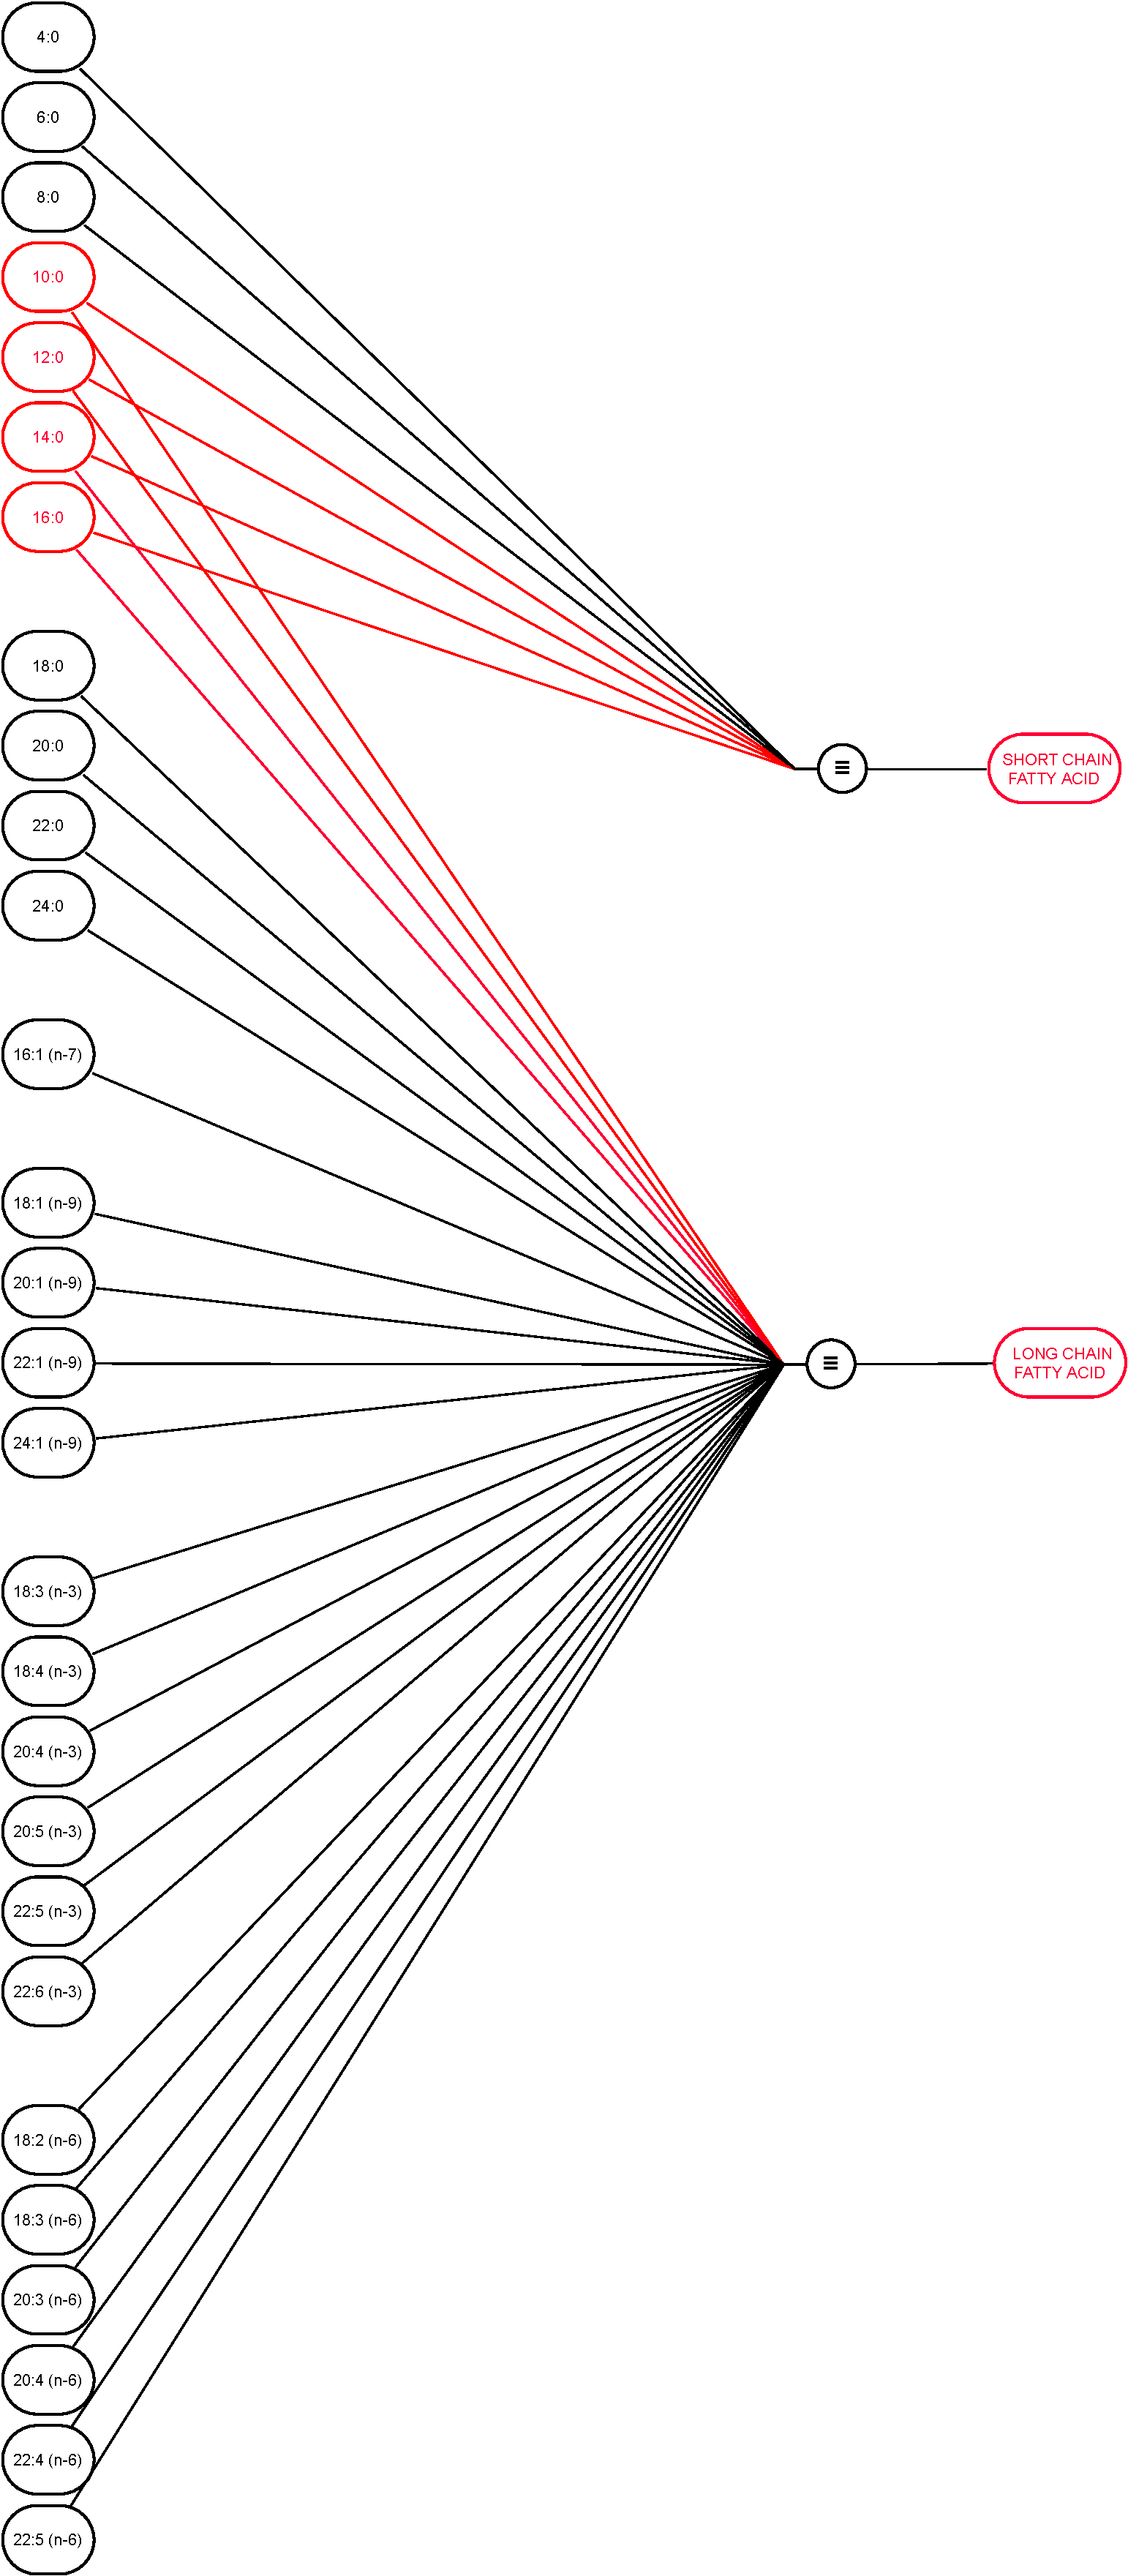
\includegraphics[scale=0.4]{examples/D3_3}
\end{center}
\caption{An example of misuse of the \glyph{equivalence operator}. The use of the \glyph{equivalence operators} does not respect the first rule, because the two generic pools colored in red on the right of the \glyph{equivalence operator} do overlap.}
\label{fig:D3_3}
\end{figure}

\begin{figure}
\begin{center}
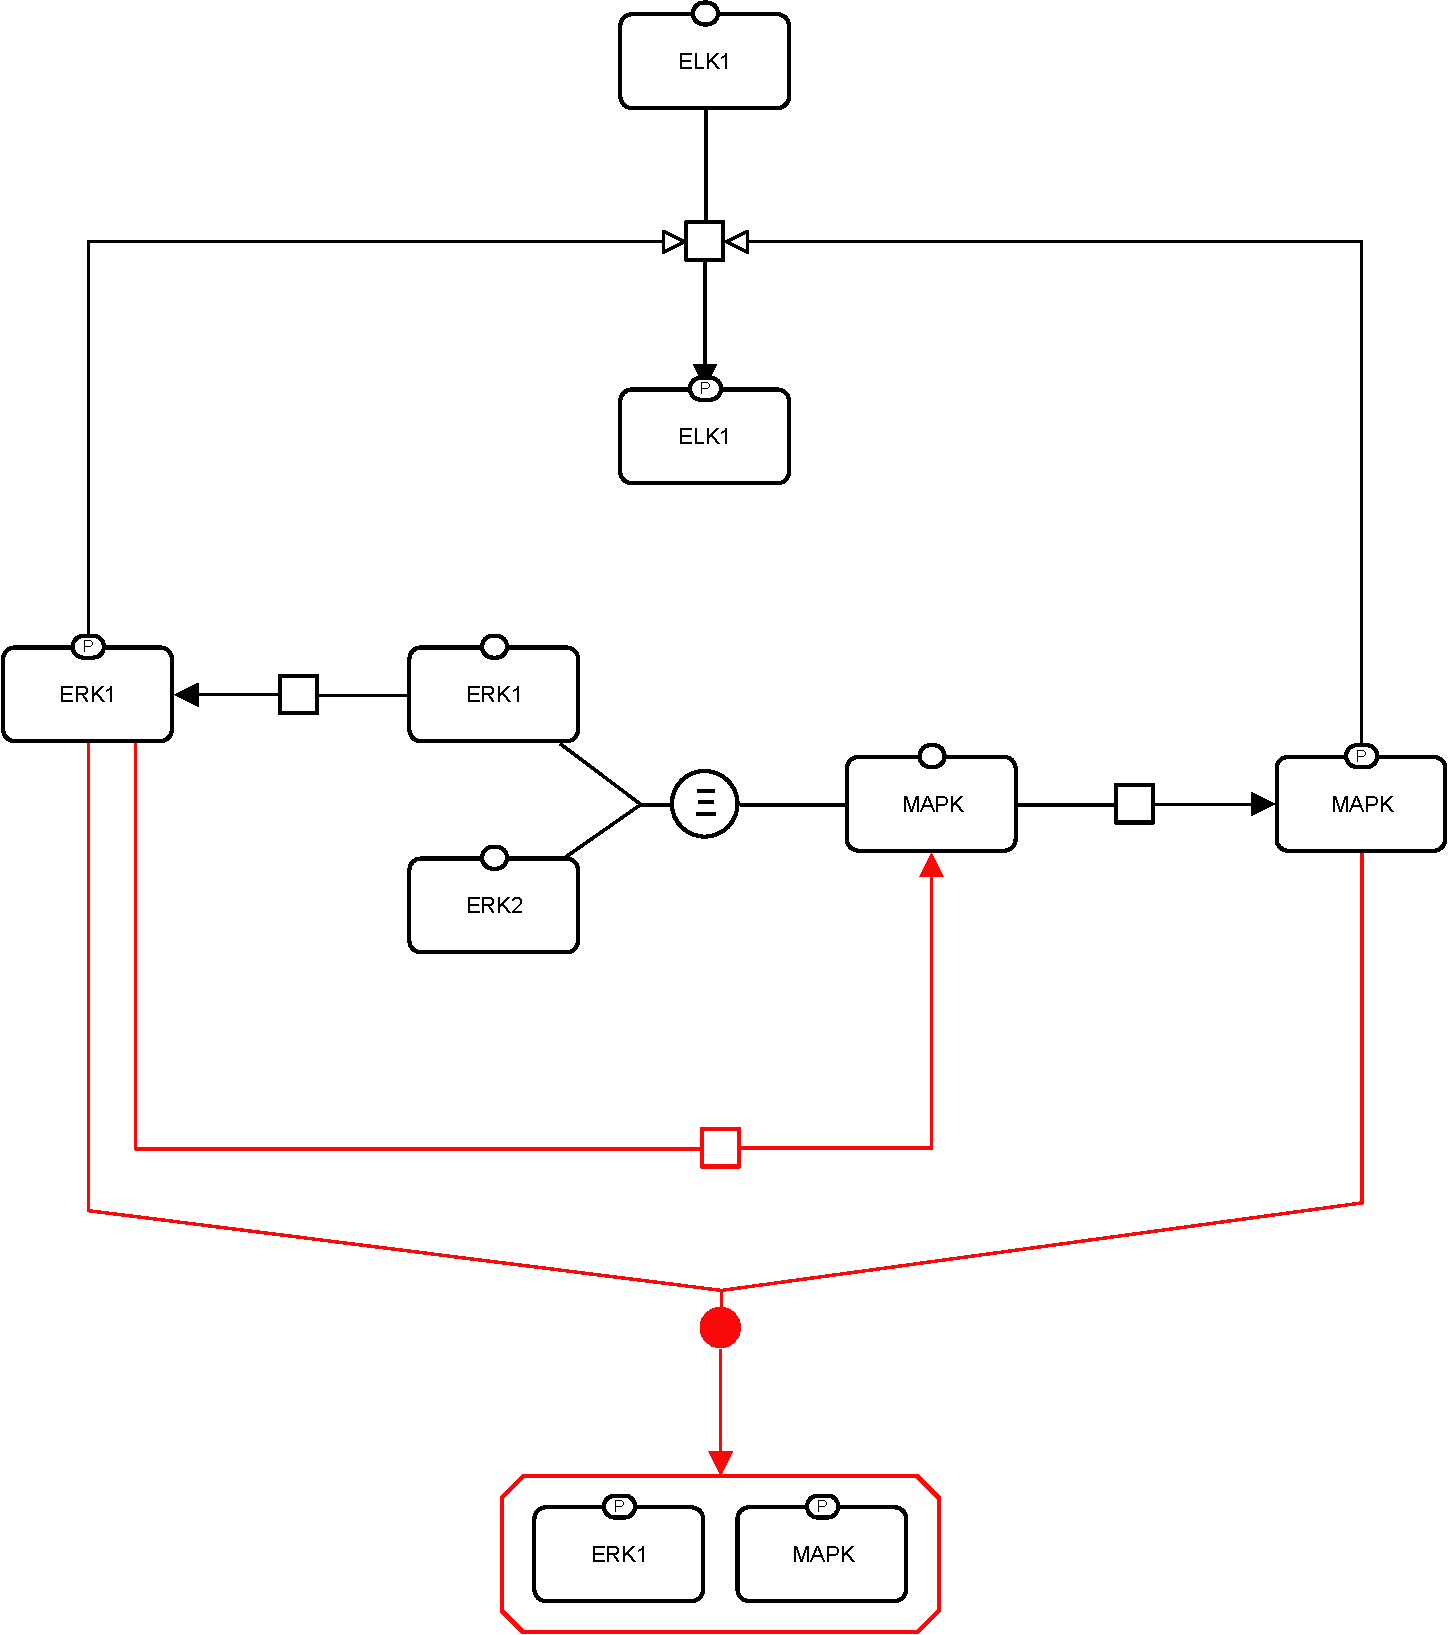
\includegraphics[scale=0.35]{examples/D3_1}
\end{center}
\caption{An example of misuse of the \glyph{equivalence operator} in a signalling pathway.
Because the phosphorylation of ERK1 is `included'' in the phosphorylation of MAPK, phosphorylated ERK1 and phosphorylated MAPK are overlapping pools, which contradicts the first rule.
As for the two processes marked in red, they both contradict the second rule, because phosphorylated ERK1 is on one side of the \glyph{equivalence operator}, while MAPK and phosphorylated MAPK are on its other side.
In terms of automatic verification, phosphorylation of MAPK can be split into two processes: phosphorylation of ERK1 and phosphorylation of ERK2 since MAPK is equivalent to ERK1 and ERK2; then there would be a repeating process of ERK1 phosphorylation.}
\label{fig:D3_1}
\end{figure}

\begin{figure}
    \centering
    \begin{tabular}{lclc}
        A & \raisebox{-\height}{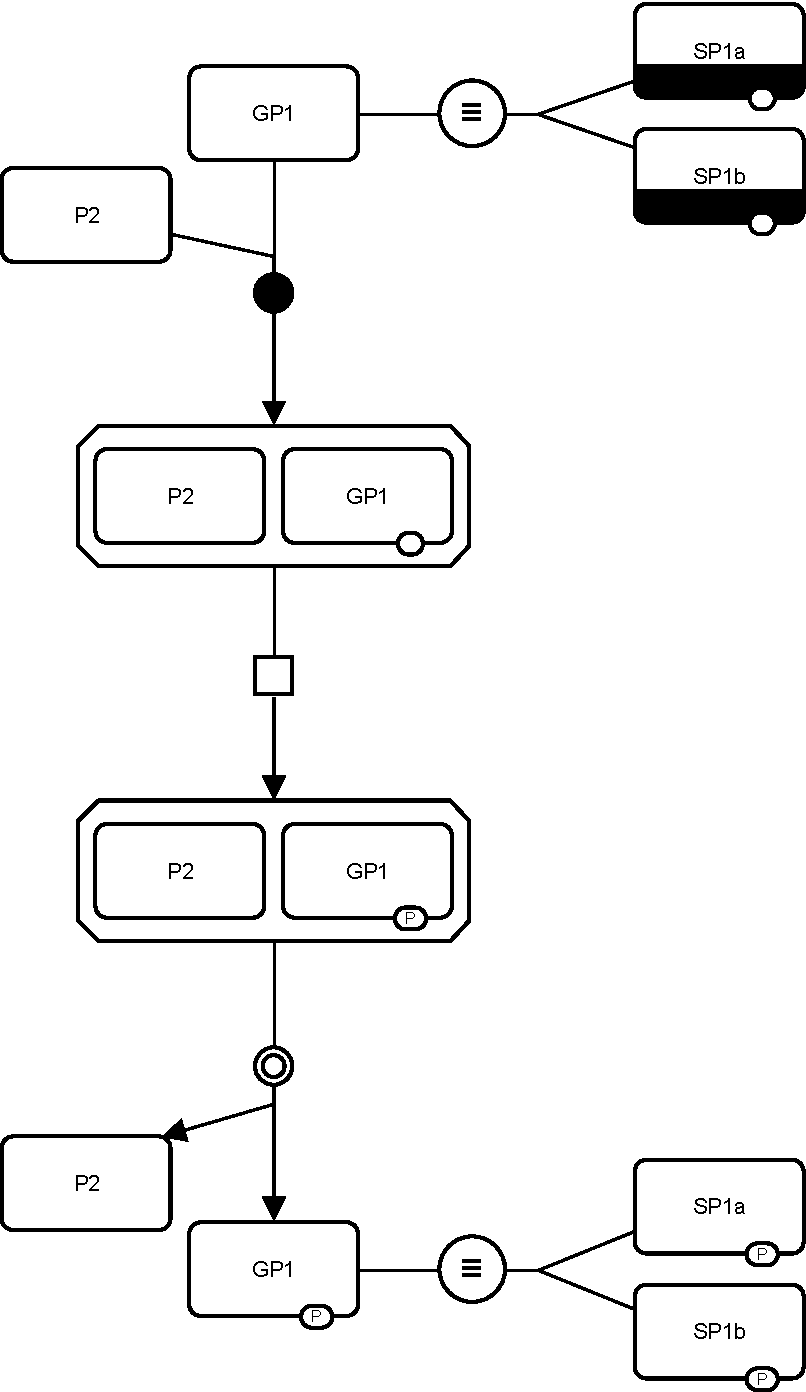
\includegraphics[scale=0.35]{examples/D3_2A}} & B & \raisebox{-\height}{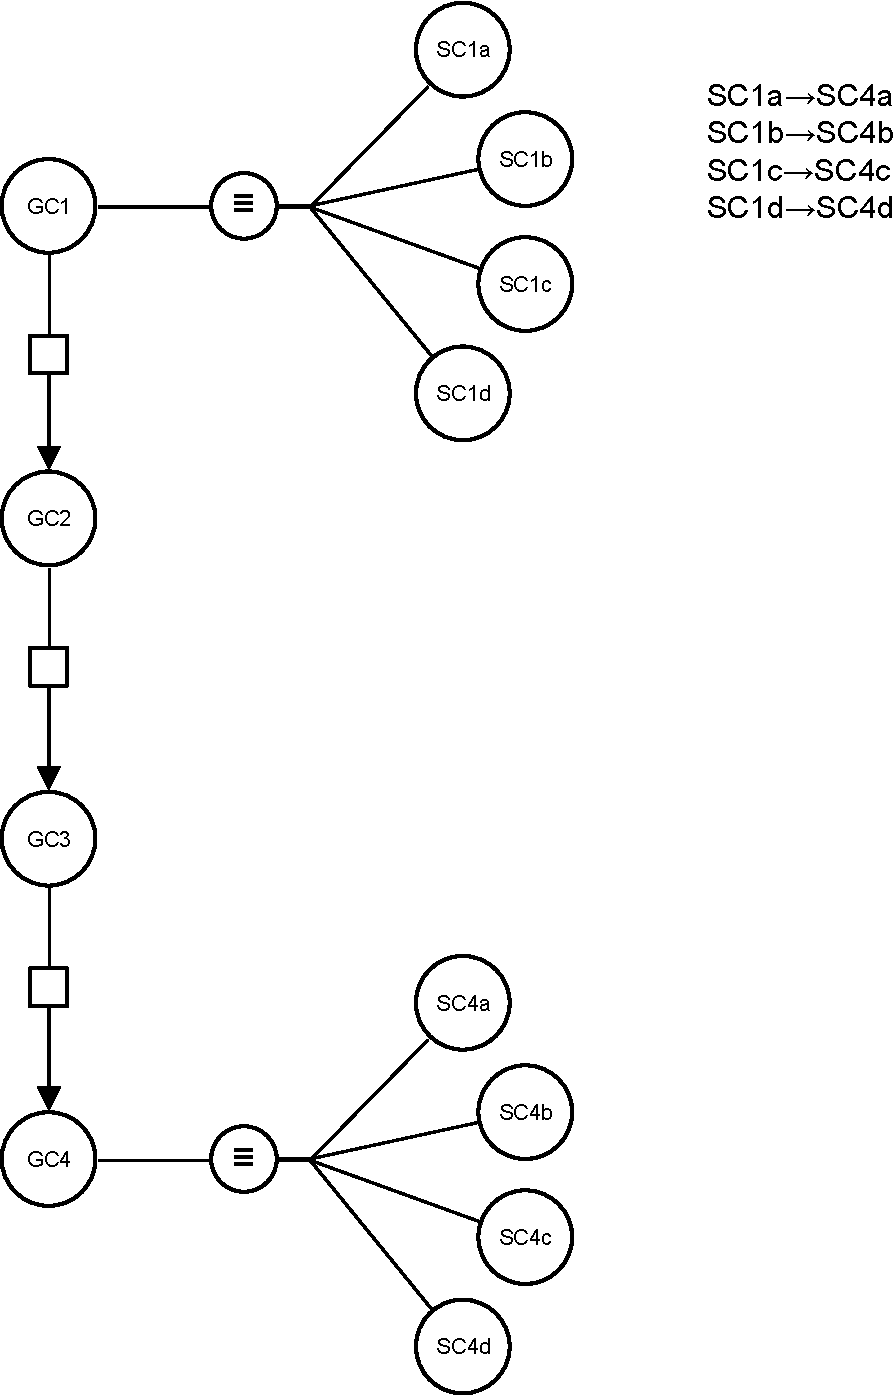
\includegraphics[scale=0.35]{examples/D3_2B}}
    \end{tabular}
\caption{An example of misuse of the \glyph{equivalence operator} in an abstract pathway involving \glyph{simple chemicals}.
A. Correct use. The use of the \glyph{equivalence operator} respects the third rule, because the pathway involves \glyph{macromolecules}, that are stateful \glyph{EPNs}.
B. Misuse. The use of the \glyph{equivalence operator} does not respect the third rule, because the pathway involves \glyph{simple chemicals}, that are stateless \glyph{EPNs}.}
\label{fig:D3_2}
\end{figure}


